%%%%%%%%%%%%%%%%%%%%%%%%%%%%%%%%%%%%%%%%%
% Beamer Presentation
% LaTeX Template
% Version 1.0 (10/11/12)
%
% This template has been downloaded from:
% http://www.LaTeXTemplates.com
%
% License:
% CC BY-NC-SA 3.0 (http://creativecommons.org/licenses/by-nc-sa/3.0/)
%
%%%%%%%%%%%%%%%%%%%%%%%%%%%%%%%%%%%%%%%%%

%----------------------------------------------------------------------------------------
%	PACKAGES AND THEMES
%----------------------------------------------------------------------------------------

\documentclass{beamer}

\mode<presentation> {

% The Beamer class comes with a number of default slide themes
% which change the colors and layouts of slides. Below this is a list
% of all the themes, uncomment each in turn to see what they look like.

%\usetheme{default}
%\usetheme{AnnArbor}
%\usetheme{Antibes}
%\usetheme{Bergen}
%\usetheme{Berkeley}
%\usetheme{Berlin}
%\usetheme{Boadilla}
%\usetheme{CambridgeUS}
%\usetheme{Copenhagen}
%\usetheme{Darmstadt}
%\usetheme{Dresden}
%\usetheme{Frankfurt}
%\usetheme{Goettingen}
%\usetheme{Hannover}
%\usetheme{Ilmenau}
%\usetheme{JuanLesPins}
%\usetheme{Luebeck}
\usetheme{Madrid}
%\usetheme{Malmoe}
%\usetheme{Marburg}
%\usetheme{Montpellier}
%\usetheme{PaloAlto}
%\usetheme{Pittsburgh}
%\usetheme{Rochester}
%\usetheme{Singapore}
%\usetheme{Szeged}
%\usetheme{Warsaw}

% As well as themes, the Beamer class has a number of color themes
% for any slide theme. Uncomment each of these in turn to see how it
% changes the colors of your current slide theme.

%\usecolortheme{albatross}
%\usecolortheme{beaver}
%\usecolortheme{beetle}
%\usecolortheme{crane}
%\usecolortheme{dolphin}
%\usecolortheme{dove}
%\usecolortheme{fly}
%\usecolortheme{lily}
%\usecolortheme{orchid}
%\usecolortheme{rose}
%\usecolortheme{seagull}
%\usecolortheme{seahorse}
%\usecolortheme{whale}
%\usecolortheme{wolverine}

%\setbeamertemplate{footline} % To remove the footer line in all slides uncomment this line
\setbeamertemplate{footline}[page number] % To replace the footer line in all slides with a simple slide count uncomment this line

%\setbeamertemplate{navigation symbols}{} % To remove the navigation symbols from the bottom of all slides uncomment this line
}

\usepackage{graphicx} % Allows including images
\usepackage{booktabs} % Allows the use of \toprule, \midrule and \bottomrule in tables
\usepackage{xcolor}% or package color
\usepackage{amssymb}
\usepackage{amsmath}
\usepackage{bm}

\graphicspath{{./Figures/}}


%----------------------------------------------------------------------------------------
%	TITLE PAGE
%----------------------------------------------------------------------------------------

\title[lab meeting]{\(r\) and \(K\) selection with genetic drift } % The short title appears at the bottom of every slide, the full title is only on the title page

\author{Freek and Ailene} % Your name

\date{\today} % Date, can be changed to a custom date

\begin{document}

\begin{frame}
\titlepage % Print the title page as the first slide
\end{frame}

\begin{frame}
\frametitle{Roughgarden 1971- Ecological model}
\begin{equation*}
N(t+1)=N(t)\left(1+r\left(1-\frac{N}{K}\right)\right)
\end{equation*}
\end{frame}

\begin{frame}
\frametitle{Roughgarden 1971- Evolutionary Model} 
\begin{figure}[H]
\centering
\begin{equation*}
N_i(t+1)=N_i(t)\begingroup\color{blue}\left(1+r_i\left(1-\frac{N_T}{K_i}\right)\right)\endgroup
\end{equation*}
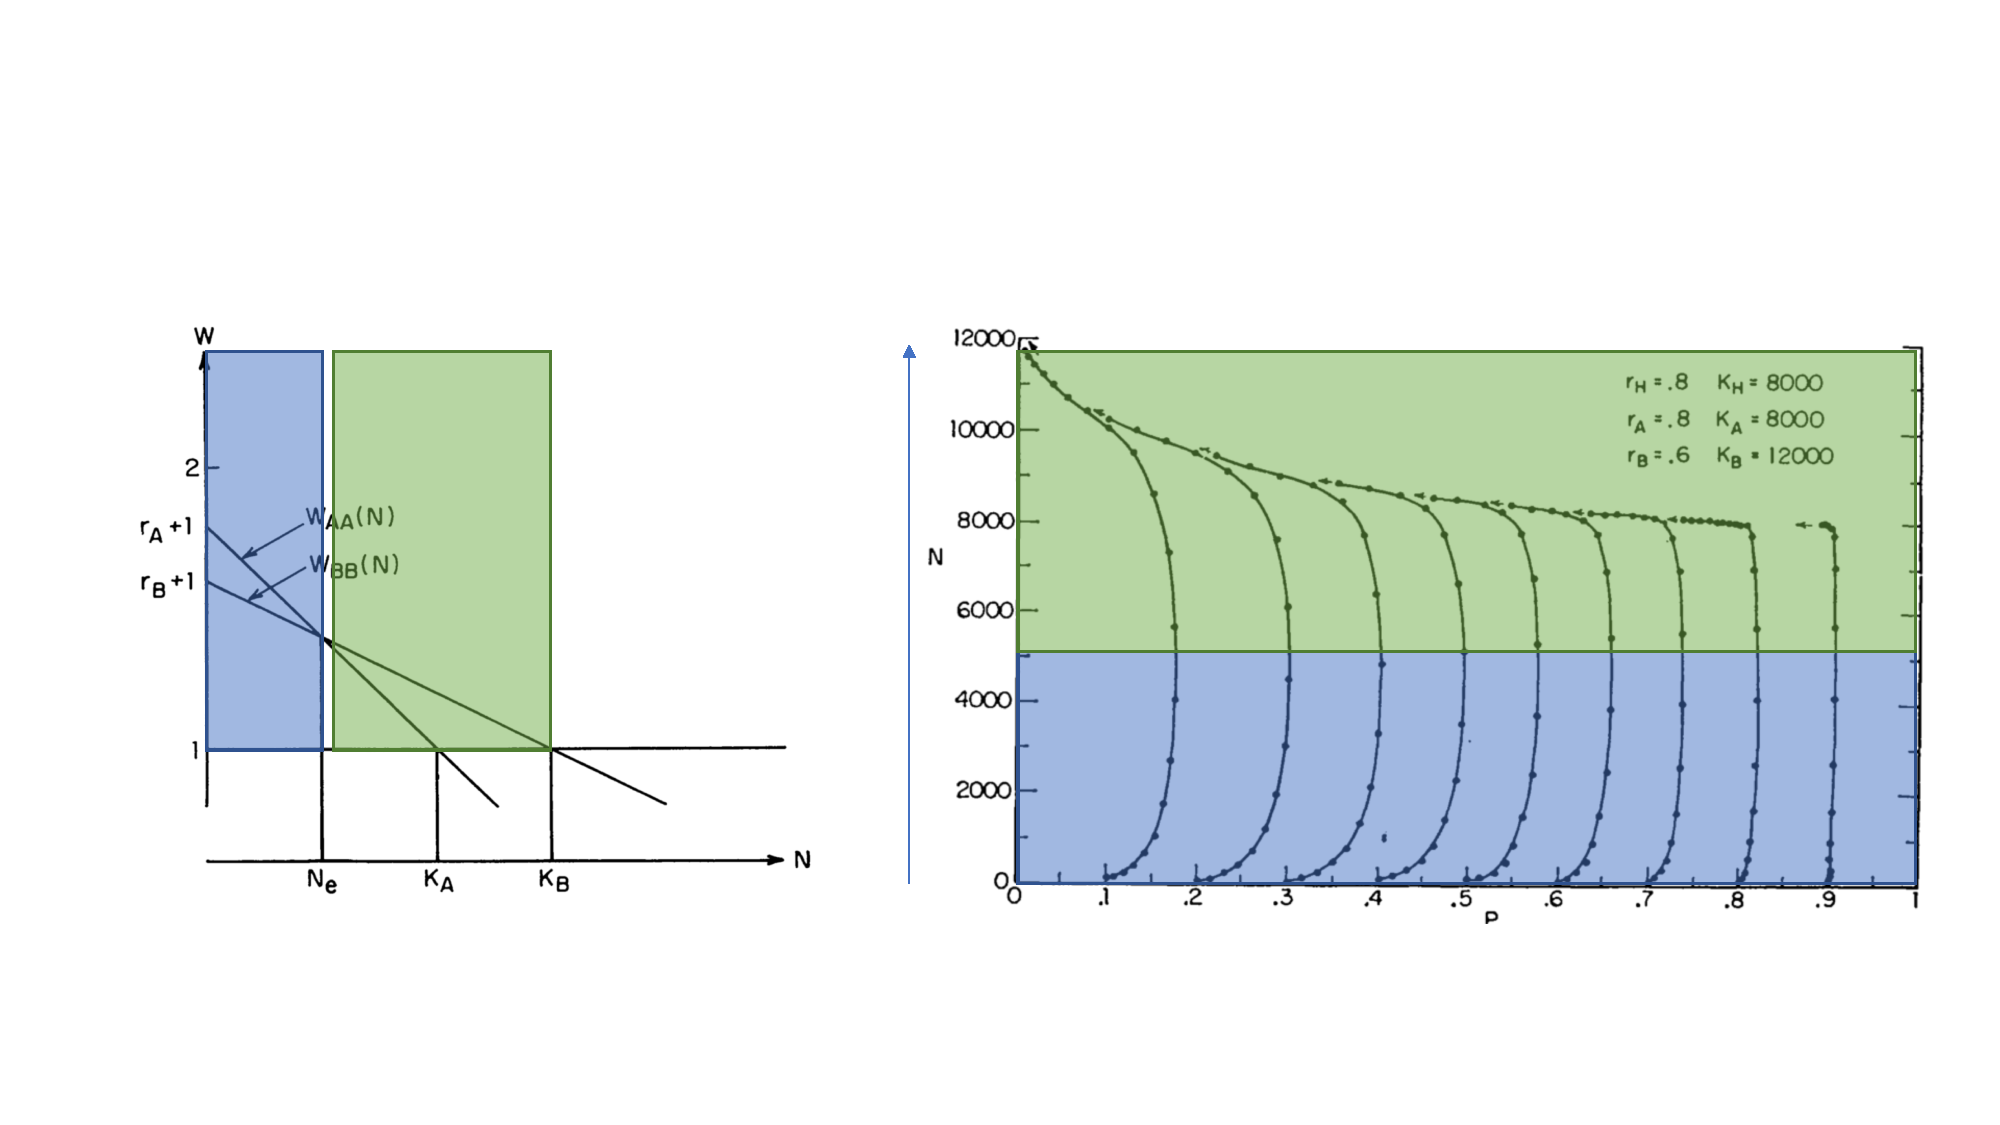
\includegraphics[width=1\textwidth]{Roughgarden.pdf}
\end{figure}
\end{frame}

\begin{frame}
\frametitle{Lande 2009- Ecological Model}
\begin{minipage}{0.45\textwidth}
\scriptsize
\begin{equation*}
\frac{dN}{dt}=\left(r\left(1-\frac{N}{K}\right)+\sigma_e\frac{dB}{dt}\right)N
\end{equation*}
Solve for the distribution of \(N\) by diffusion.\newline\newline
But first we must transform \(N\)
\begin{equation*}
\frac{dln(N)}{dt}=\left(r\left(1-\frac{N}{K}\right)+\sigma_e\frac{dB}{dt}\right)\begingroup\color{red}-\frac{\sigma_e^2}{2}\endgroup
\end{equation*}
\normalsize
\end{minipage}
\begin{minipage}{0.45\textwidth}
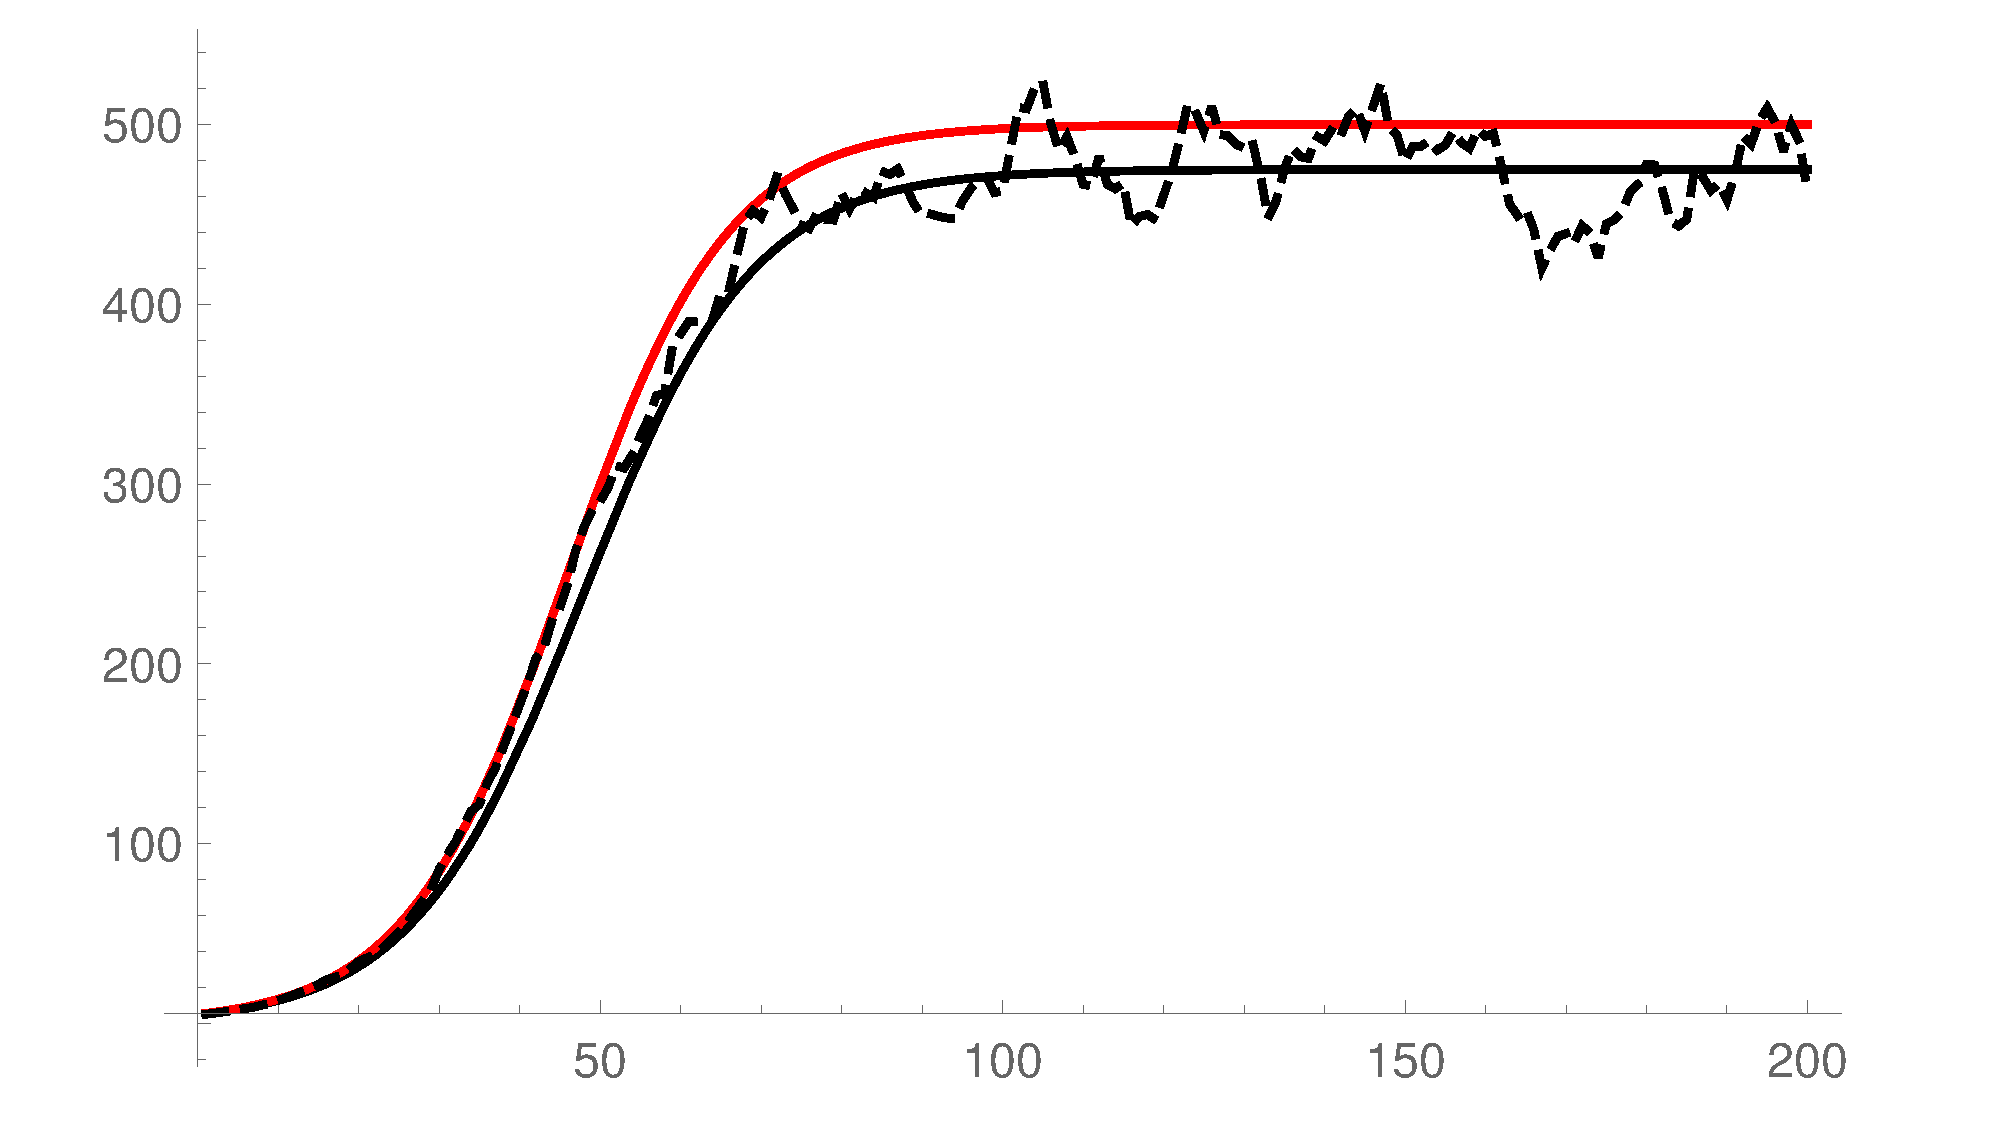
\includegraphics[width=1.2\columnwidth]{Itoprocess.pdf}
\end{minipage}
\end{frame}

\begin{frame}
\frametitle{Ito's Lemma and Stochastic DEs}
If \(X(t)\) is an Ito process
\begin{equation}
\label{X(t)}
\frac{dX}{dt}=\mu+\sigma\frac{dB}{dt}
\end{equation}
A function of a stochastic process $C=f(X(t),t)$.  \(C\) is also a Ito process
\begin{equation}
\frac{df}{dt}\approx\frac{df}{dt}+\frac{df}{dx}\frac{dx}{dt}+\frac{1}{2}\frac{d^2f}{dx^2}(dx)^2
\end{equation}
Plugging in \eqref{X(t)} we have
\begin{equation}
\frac{df}{dt}\approx\frac{df}{dt}+\mu\frac{df}{dx}+\begingroup\color{red}\frac{\sigma^2}{2}\frac{d^2f}{dx^2}\endgroup+\sigma\frac{df}{dx}\frac{dB}{dt}
\end{equation}
\textcolor{red}{Only matters for non-linear \(f(x)\)}
\end{frame}

\begin{frame}
\frametitle{Lande 2009-Ecological model}
\begin{minipage}{0.45\textwidth}
\scriptsize
\begin{equation*}
\begin{aligned}
 \frac{dN}{dt}&=\left(r\left(1-\frac{N}{K}\right)+\sigma_e\frac{dB}{dt}\right)N\\
\frac{dln(N)}{dt}&=\left(r\left(1-\frac{N}{K}\right)+\sigma_e\frac{dB}{dt}\right)\begingroup\color{red}-\frac{\sigma_e^2}{2}\endgroup\\
\end{aligned}
\end{equation*}
Solving for the diffusion moments
\begin{equation*}
\begin{aligned}
E[\frac{dln(N)}{dt}]&=r\left(1-\frac{N}{K}\right)-\frac{\sigma_e^2}{2}\\
Var[\frac{dln(N)}{dt}]&=\sigma_e^2
\end{aligned}
\end{equation*}
\normalsize
\end{minipage}
\begin{minipage}{0.45\textwidth}
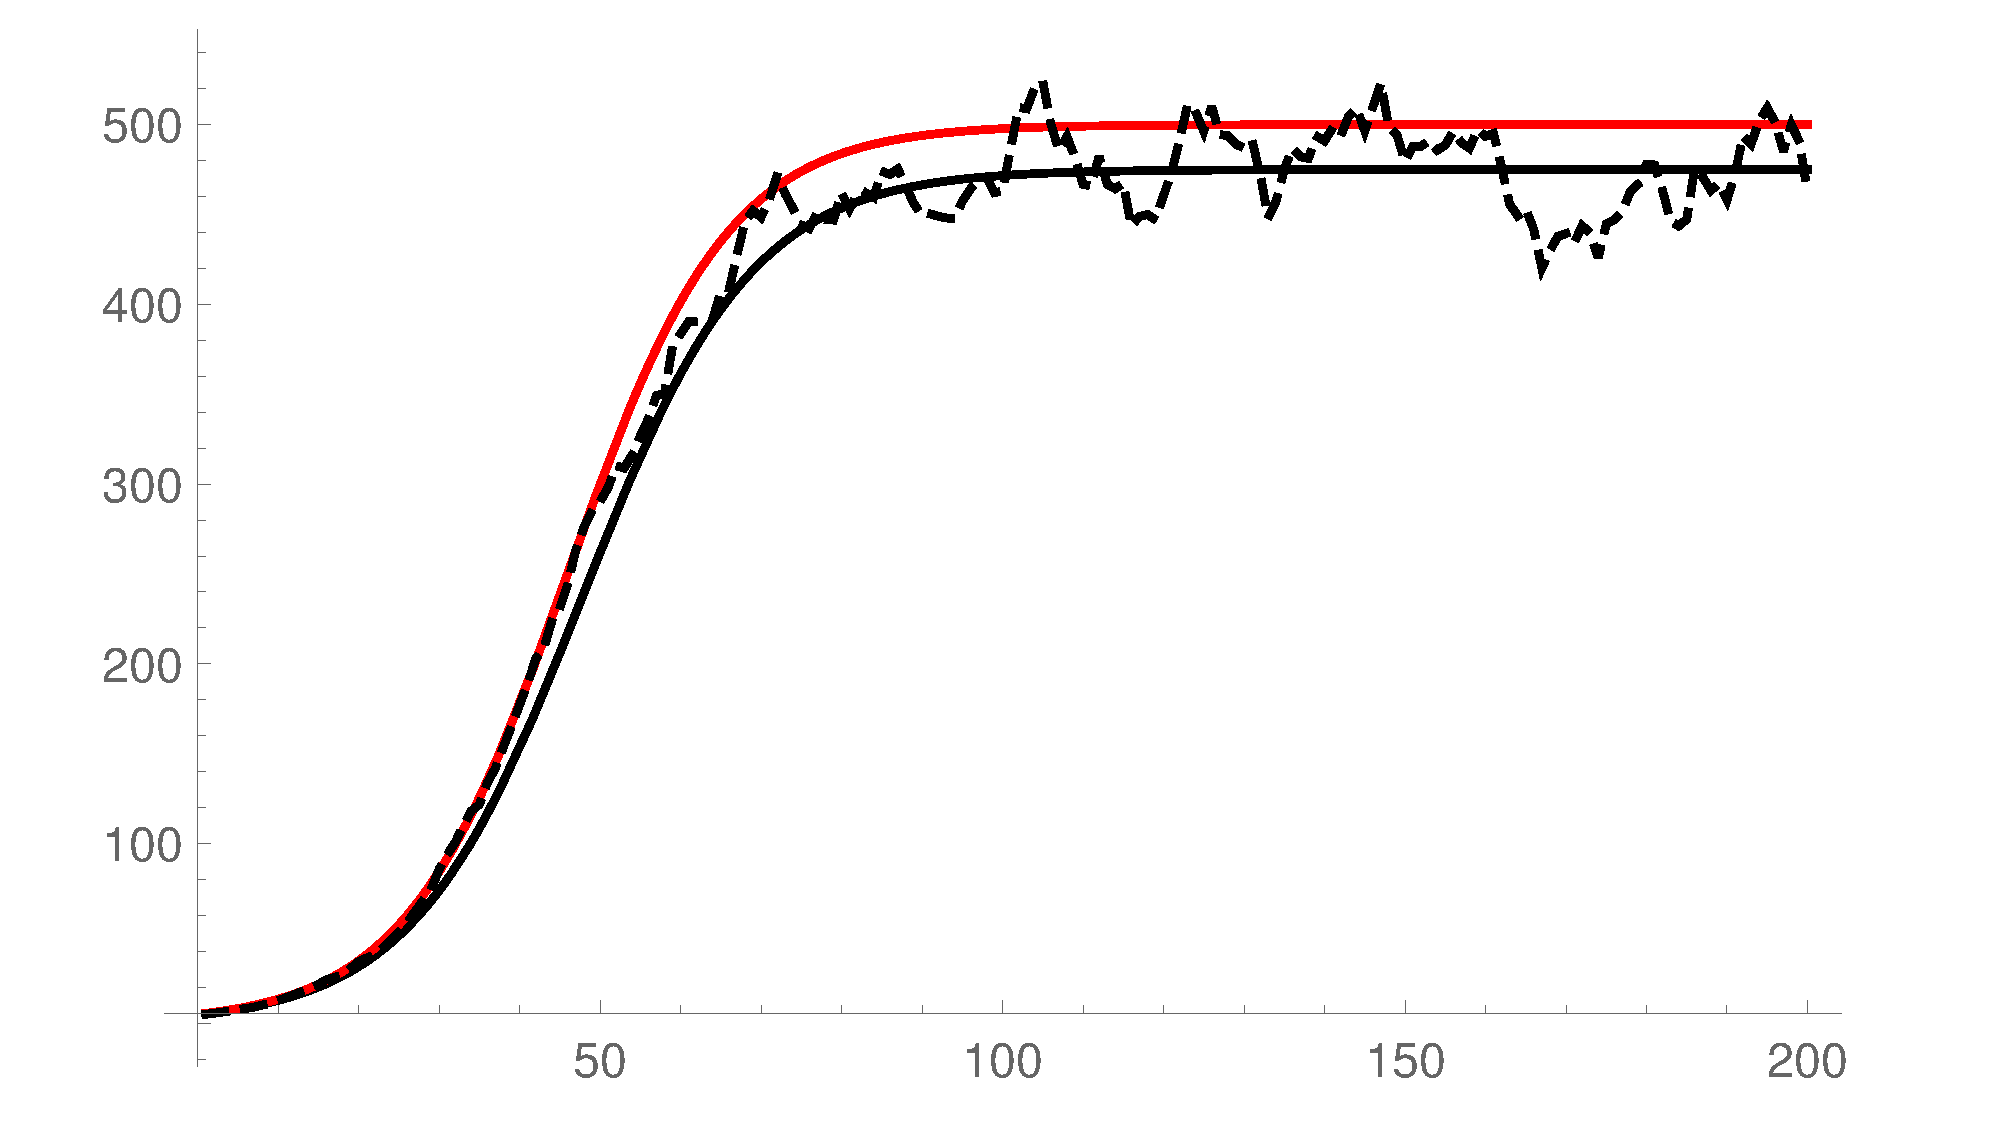
\includegraphics[width=1.2\columnwidth]{Itoprocess.pdf}
\end{minipage}%
\end{frame}

\begin{frame}
\frametitle{Lande 2009- Evolutionary Model}
\begin{equation*}
\frac{dN_i}{dt}=\left(r_i-g_i(N_T)+\begingroup\color{red}c_{i,i}\frac{dB_i}{dt}\endgroup\right)N_i
\end{equation*}
Solve 2 ways:\newline
1) Diffusion Approximation\newline
2) Invasion Analysis
\end{frame}

\begin{frame}
\frametitle{Lande 2009- Diffusion solution}
\begin{equation*}
\frac{dN_i}{dt}=\left(r_i-g_i(N_T)+\begingroup\color{red}c_{i,i}\frac{dB_i}{dt}\endgroup\right)N_i
\end{equation*}
\begin{center}
Transform into \(ln(N_T)\) and \(p\)
\end{center}
\scriptsize
\begin{equation*}
\begin{aligned}
&E[\frac{d ln(N_T)}{dt}]=\left(\bar{r}-\bar{g}(N_T)-\frac{\sigma_e^2}{2}\right)\quad\text{Var}[\frac{d ln(N_T)}{dt}]=\sigma_e^2 \\
&E[\frac{dp}{dt}]=p(1-p) \frac{\partial}{\partial p} \begingroup\color{blue}\left(\bar{r}-\bar{g}(N_T)-\frac{\sigma_e^2}{2}\right)\endgroup\\
&\text{Var}[\frac{dp}{dt}=\frac{p^2(1-p^2)}{2}\frac{\partial^2 \sigma^2}{\partial p^2}\quad\text{Cov}[\frac{dp}{dt},\frac{dln(N_T)}{dt}]=\frac{p(1-p)}{2}\frac{\partial \sigma^2}{\partial p}
\end{aligned}
\end{equation*}
\normalsize
\end{frame}

% \begin{frame}
% \frametitle{Lande 2009- Diffusion solution}
% \begin{minipage}{0.45\textwidth}
% \begin{center}
% Infinitesimal moments
% \end{center}
% \footnotesize
% \begin{equation*}
% \begin{aligned}
% &E[\frac{d ln(N_T)}{dt}]=\left(\bar{r}-\bar{g}(N_T)-\frac{\sigma_e^2}{2}\right) \\
% &\text{Var}[\frac{d ln(N_T)}{dt}]=\sigma_e^2 \\
% &E[\frac{dp}{dt}]=p(1-p) \frac{\partial}{\partial p} \begingroup\color{red}\left(\bar{r}-\bar{g}(N_T)-\frac{\sigma_e^2}{2}\right)\endgroup\\
% &\text{Var}[\frac{dp}{dt}=\frac{p^2(1-p^2)}{2}\frac{\partial^2 \sigma^2}{\partial p^2}\\
% &\text{Cov}[\frac{dp}{dt},\frac{dln(N_T)}{dt}]=\frac{p(1-p)}{2}\frac{\partial \sigma^2}{\partial p}
% \end{aligned}
% \end{equation*}
% \normalsize
% \end{minipage}
% \hfill
% \begin{minipage}{0.45\textwidth}
% \scriptsize
% \(\bar{r}\): average growth rate\newline
% \begin{equation*}
% \bar{r}=p r_1+q r_2
% \end{equation*}
% \(\bar{g}(N_T)\): average density dependence\newline
% \begin{equation*}
% \bar{g}(N_T)=p g_1(N_T)+q g_2(N_T)
% \end{equation*}
% \(\sigma_e\): average stochasticity\newline
% \begin{equation*}
% \bar{g}(N_T)=p^2 c_{1,1}+2pq c_{1,2}+q^2 c_{2,2}
% \end{equation*}
% \normalsize
% \end{minipage}%
% \end{frame}

\begin{frame}
\frametitle{Lande 2009-Invasion analysis}
What if \(r_i\) and \(g_i(N_T)\) are not independent?
\begin{equation*}
g_i(N_T)=\frac{r_i}{K_i}N_t
\end{equation*}
Mutant fitness given resident \(N_R\)
\begin{equation*}
W_m=E[\frac{dln(N_m)}{dt}]=r_m\left(1-\frac{N_R}{K_m}\right)-\frac{c_{m,m}^2}{2}
\end{equation*}
Average over distribution of \(N_R\) gives invasion criteria:
\begin{equation*}
\begin{aligned}
r_m\left(1-\frac{\begingroup\color{red}E[N_R]\endgroup}{K_m}\right)-\frac{c_{m,m}^2}{2} > 0 \\
\begingroup\color{blue}(1-\frac{c_{m,m}^2}{2r_m})K_m\endgroup > (1-\frac{c_{R,R}^2}{2r_R})K_R
\end{aligned}
\end{equation*}
\end{frame}

\begin{frame}
\frametitle{Lande 2009- Numerical example}
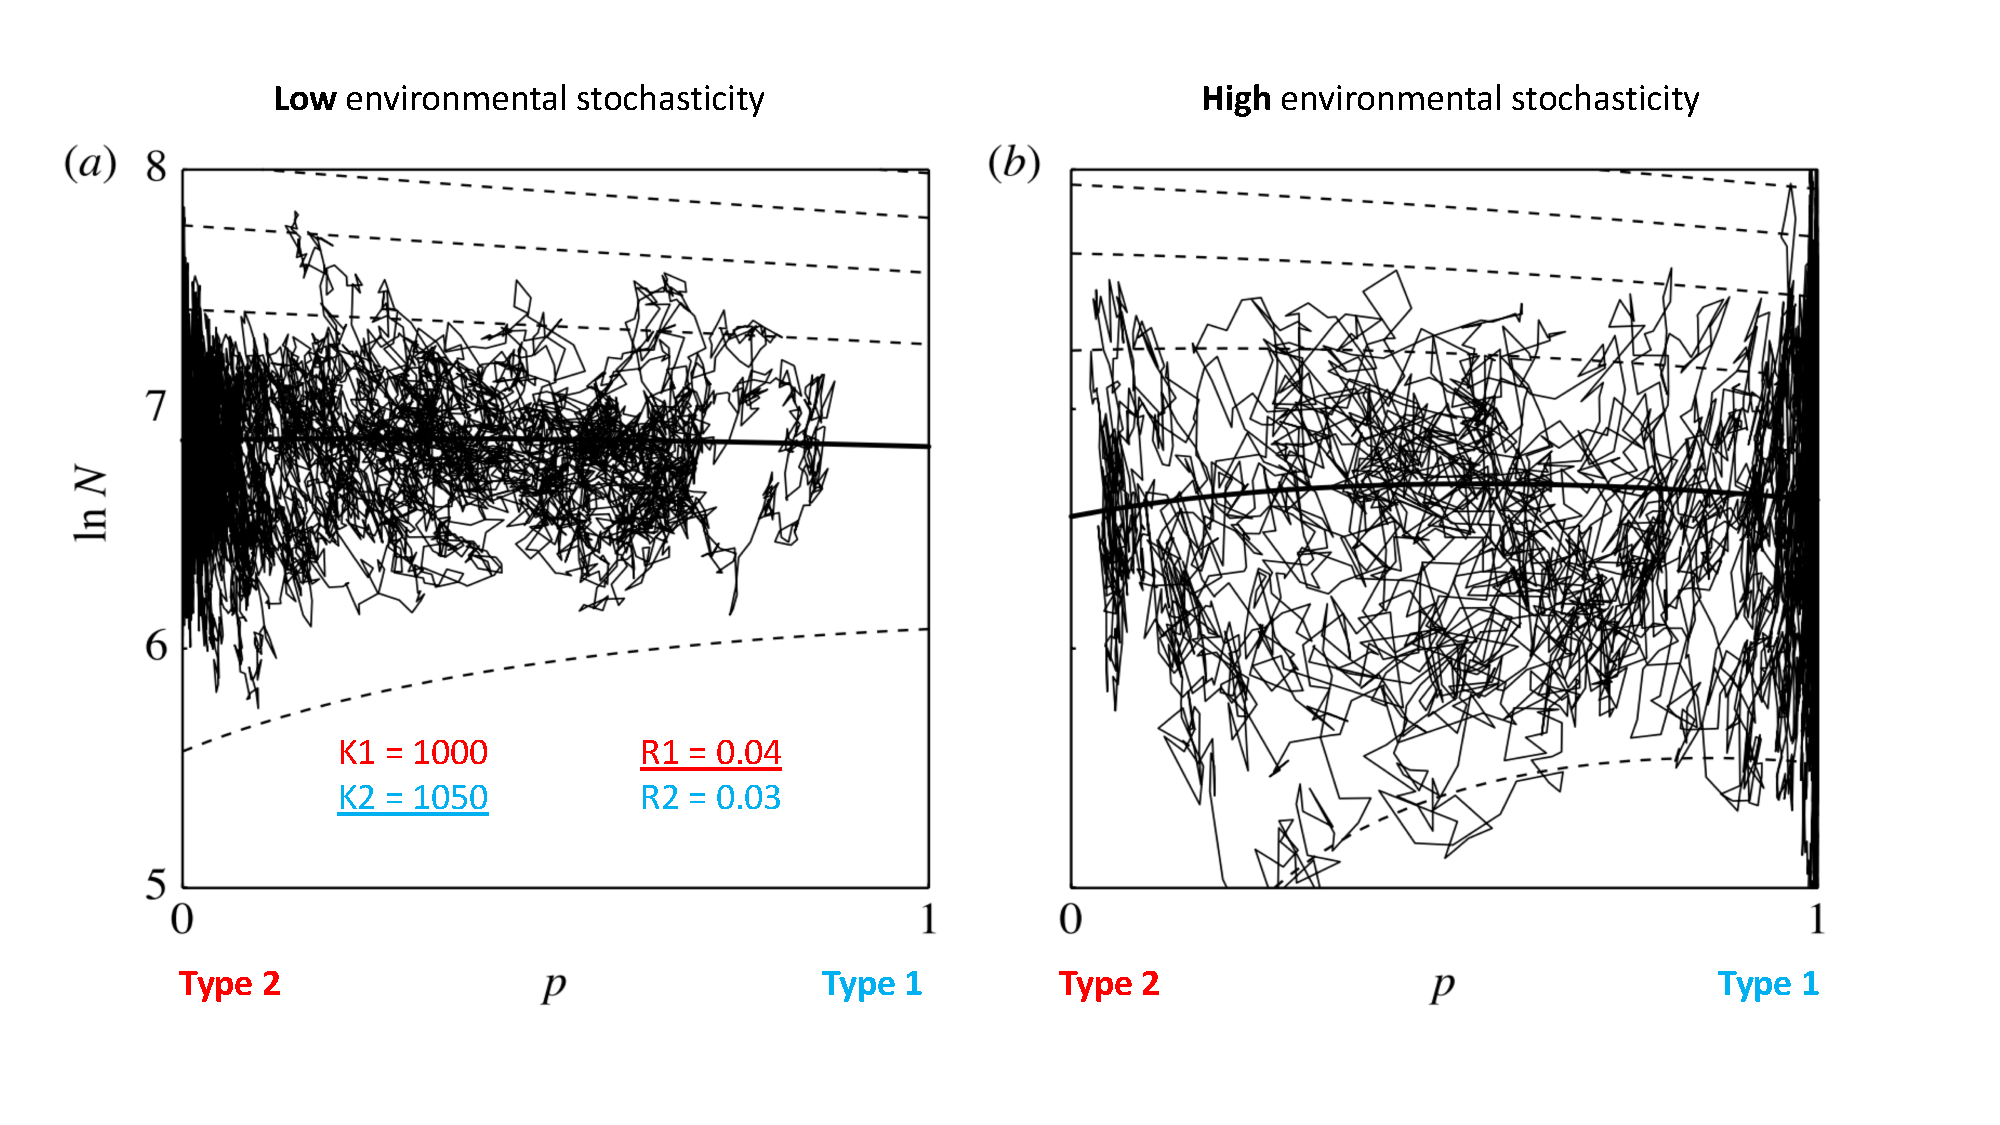
\includegraphics[width=\columnwidth]{LandeNumeric.pdf}
\end{frame}

\begin{frame}
\frametitle{Engen 2013- Ecological Model}
\begin{center}
Same as Lande 2009...almost
\end{center}
\begin{equation*}
\frac{d N}{dt}=\left(r+\begingroup\color{red}\gamma\endgroup g(N)+\sigma_e\frac{dB}{dt}\right)N
\end{equation*}
\end{frame}

\begin{frame}
\frametitle{Engen 2013- Evolutionary Model}
\begin{center}
A quantitative genetics version of Lande 2009...almost

\begin{equation*}
\frac{d N(z)}{dt}=\left(r(z)+\begingroup\color{red}\gamma(z)\endgroup g(N_T)+c(z,z)\frac{dB}{dt}\right)N(z)
\end{equation*}
Transform into \(ln(N_T)\) and the distribution of \(z\)
\scriptsize
\begin{equation*}
\begin{aligned}
&E[\frac{d ln(N_T)}{dt}]= \bar{r}(\bar{z})-\bar{\gamma}(\bar{z})g(N_T) -\frac{1}{2}\sigma_e(\bar{z})^2\quad \text{Var}[\frac{d ln(N_T)}{dt}]= \sigma_e^2\\
&E[\frac{dz}{dt}]= G \frac{\partial}{\partial \bar{z}}\begingroup\color{blue}\left(\bar{r}(\bar{z})-\bar{\gamma}(\bar{z})g(N_T)\right)-\frac{1}{2}\sigma_e(\bar{z})^2\endgroup\\
&\text{Var}[\frac{dz}{dt} ]= \text{Mess A} \quad\text{Cov}[\frac{dz}{dt},\frac{dln(N_T)}{dt}]= \text{Mess B} 
\end{aligned}
\end{equation*}
\normalsize
\end{center}
\end{frame}

% \begin{frame}
% \frametitle{Background-Engen 2013}
% Evolution maximizes
% \begin{equation*}
% \left(\bar{r}(\bar{z})-\bar{\gamma}(\bar{z})g(N_T)\right)-\frac{1}{2}\sigma_e(\bar{z})^2
% \end{equation*}
% This is a function of \(z\) and \(N_T\), how does \(z\) evolve?
% \begin{equation*}
% g(N_T)=\frac{\bar{s}(\bar{z})}{\bar{\gamma}(\bar{z})}
% \end{equation*}
% So evolution maximizes:
% \begin{equation*}
% (1-\frac{\sigma(\bar{z})^2}{2\bar{r}(\bar{z})})g(K(\bar{z}))
% \end{equation*}
% \end{frame}

% \begin{frame}
% \frametitle{Background-Engen 2013}
% \begin{equation*}
% m(z,N)=r(z)-\gamma(z)g(N)
% \end{equation*}
% $r(z)$ governs the strength of \textit{density independent} selection, and $\gamma(z)$ the density \textit{dependent} part.
% \begin{equation*}
% E[\frac{dz}{dt}]= \bar{\gamma}(\bar{z}) \frac{\partial}{\partial t} \frac{\bar{s}(\bar{z})}{\bar{\gamma}(\bar{z})}
% \end{equation*}
% Which shows that evolution optimizes the following equality, similar to Lande:
% \begin{equation*}
% (1-\frac{\sigma(\bar{z})^2}{2\bar{r}(\bar{z})})g(K(\bar{z}))
% \end{equation*}
% \end{frame}

\begin{frame}
\frametitle{Engen 2013- Numerical example}
\begin{minipage}{0.45\textwidth}
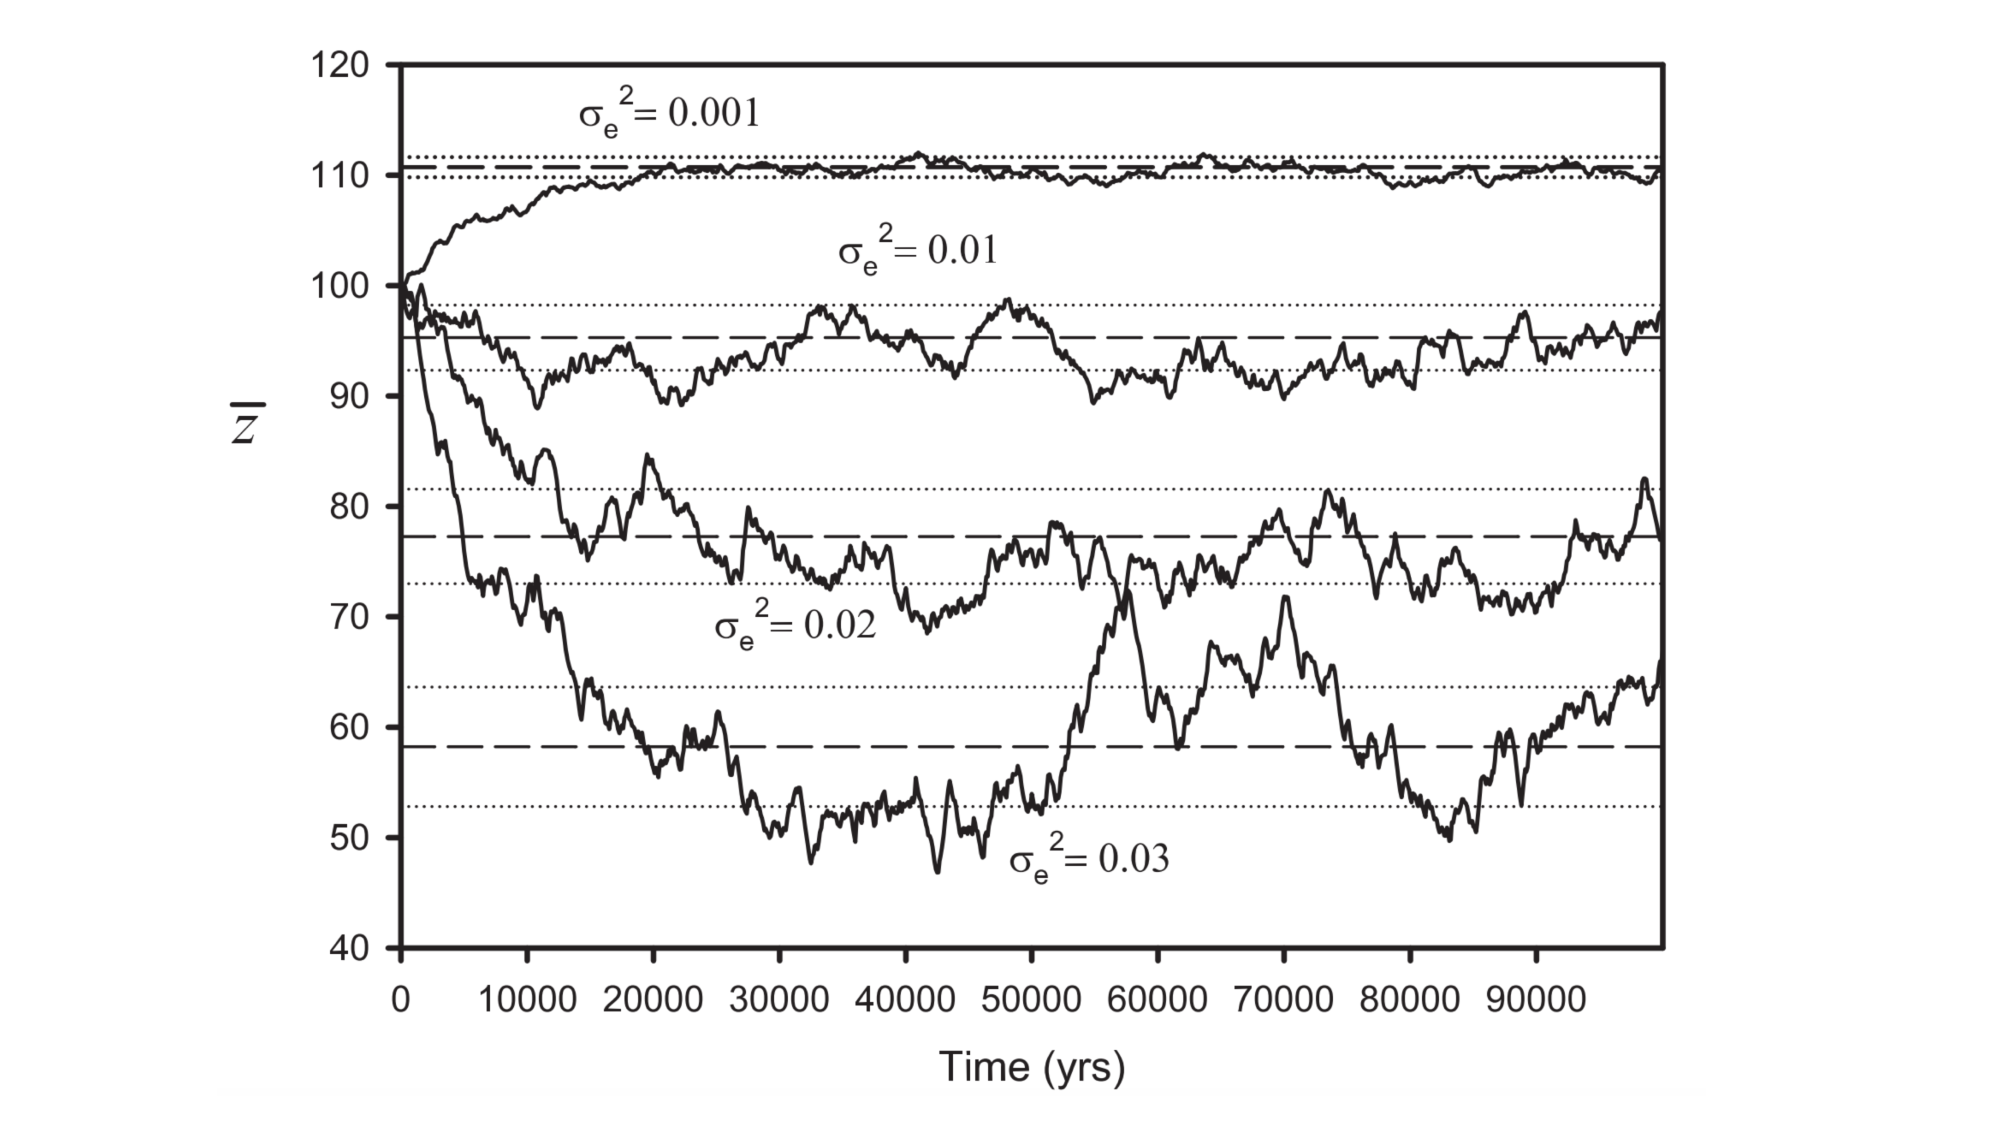
\includegraphics[width=1.2\columnwidth]{Engen.pdf}
\end{minipage}%
\hfill
\begin{minipage}{0.45\textwidth}
They propose a \textbf{trade-off}:
\begin{equation*}
\begin{aligned}
r(z)=r_0(1-e^{\alpha(z-z_0)}) \\
\gamma(z)= \frac{r(z)}{K(z)} =\gamma_0 e^{-\beta z}
\end{aligned}
\end{equation*}
Which are 2 decreasing functions with increasing $z$.
\end{minipage}%
\end{frame}

\begin{frame}
\frametitle{Environmental Stochasticity vs. Genetic Drift}
Environmental Stochasticity
\begin{equation*}
\frac{dn_i}{dt}=n_i\left(r_i(1-\frac{n_T}{K_i})+\begingroup\color{red}\frac{dB}{dt}\endgroup\right)
\end{equation*}
Genetic Drift
\begin{equation*}
\frac{dN_i}{dt}=N_i\left(r_i\left(1-\frac{N_T}{K_i}\right)\right)+\begingroup\color{red}\frac{dB}{dt}\endgroup
\end{equation*}
\end{frame}
\begin{frame}
\frametitle{Ecological Model (No evolution)}
Deterministic Model
\begin{equation*}
N'=\begingroup\color{blue}N r\left(1-\frac{N}{\gamma}\right)\endgroup \color{green}s+\color{purple}m
\end{equation*}
Stochastic Model
\begin{equation*}
\pmb{T}=\color{purple}\pmb{M}\color{green}\pmb{D}\color{blue}\pmb{B}
\end{equation*}
\tiny
\begin{center}
Probability of going from \(i\) to \(j\)
\end{center}
\begin{equation*}
\begin{aligned}
B_{j,i}&=\begin{cases}
\mathcal{P}\left(i r(1-\frac{i}{\gamma}),j-i\right)& i\leq j\leq n_{Max}\\
0 & \text{otherwise}
\end{cases}\\
D_{j,i}&=\mathcal{B}\left(i,s,j\right)\\
M_{j,i}&=\begin{cases}
\mathcal{P}\left(m,j-i\right)& i\leq j\leq n_{Max}\\
0 & \text{otherwise}
\end{cases}\\
\end{aligned}
\end{equation*}
\normalsize
\end{frame}
\begin{frame}
\frametitle{Ecological Dynamics}
\begin{center}
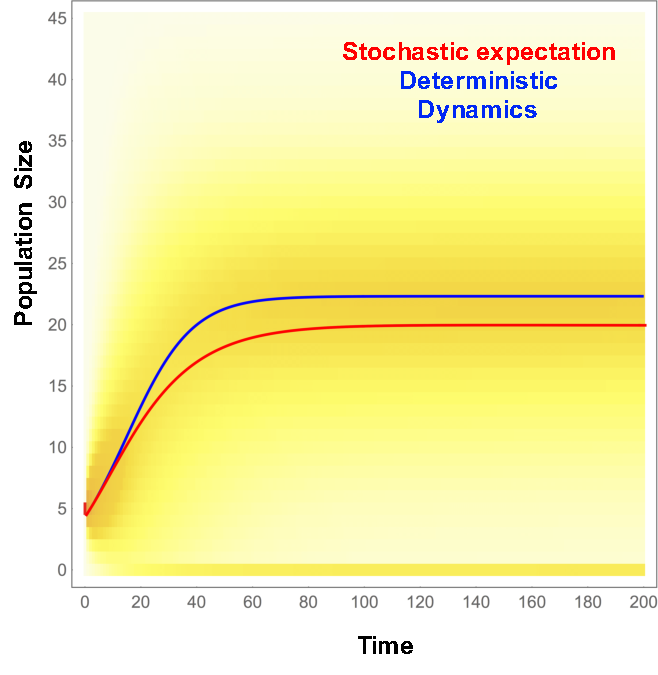
\includegraphics[width=0.6\textwidth]{ecoModel.pdf}
\end{center}
\end{frame}
\begin{frame}
\frametitle{Evolutionary Models}
Density-independent \textbf{selection} Model
\begin{equation*}
\begin{aligned}
n_i(t+1)&=\begingroup\color{blue}n_i(t)r\left(1-\frac{n_T(t)}{\gamma}\right)\endgroup \begingroup\color{green}\pmb{s_i}\endgroup+\color{purple}m\\
w_i&=f(p)
\end{aligned}
\end{equation*}
Density-dependent \textbf{selection} Model
\begin{equation*}
\begin{aligned}
N_i(t+1)&=\begingroup\color{blue}N_i(t)\pmb{r_i}\left(1-\frac{N_T(t)}{\pmb{\gamma_i}}\right)\endgroup \begingroup\color{green}s\endgroup+\begingroup\color{purple}m\endgroup\\
r_i\gamma_i^\frac{1}{\pmb\beta}&=\text{constant}\\
w_i&=f(N_T,p)
\end{aligned}
\end{equation*}
\end{frame}

\begin{frame}
\frametitle{Density-independent Model}
\begin{minipage}{0.45\textwidth}
\tiny
\begin{center}
\end{center}
\begin{equation*}
\begin{aligned}
B_{(j_1,j_2),(i_1,i_2)}&=\mathcal{P}\left(i_1 r(1-\frac{i_1+i_2}{\gamma}),j_1-i_1\right)\\
&*\mathcal{P}\left(i_2 r(1-\frac{i_1+i_2}{\gamma}),j_2-i_2\right)\\
D_{(j_1,j_2),(i_1,i_2)} &=\mathcal{B}\left(i_1,s_1,j_1\right)*\mathcal{B}\left(i_2,s_2,j_2\right)\\
M_{(j_1,j_2),(i_1,i_2)} &=\mathcal{P}\left(m,j_1-i_1\right)\\
&*\mathcal{P}\left(m,j_2-i_2\right)
\end{aligned}
\end{equation*}
Poisson only valid when \(i_1\leq j_1, i_2\leq j_2\)
\normalsize
\end{minipage}%
\begin{minipage}{0.45\textwidth}
\begin{center}
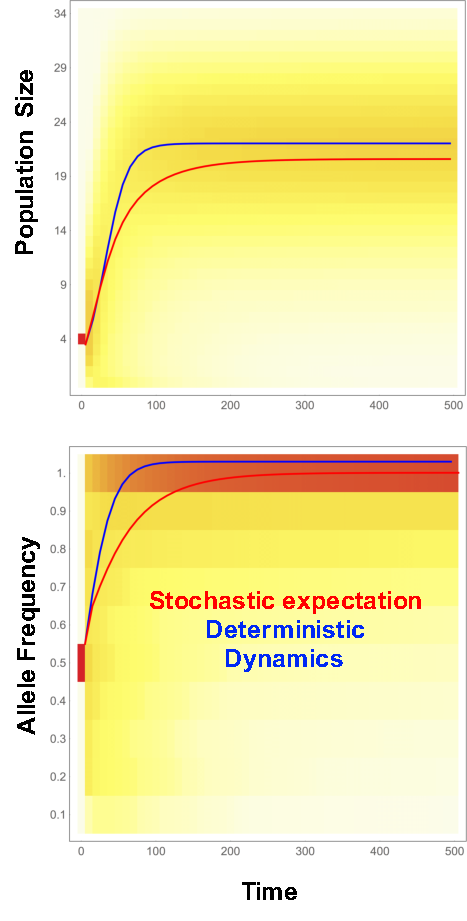
\includegraphics[width=0.7\columnwidth]{DensityIndependent.pdf}
\end{center}
\end{minipage}%
\end{frame}

\begin{frame}
\begin{center}
\includegraphics[width=0.7\columnwidth]{sparse.png}
\end{center}
\end{frame}

\begin{frame}
\frametitle{Density-dependent Model}
\begin{minipage}{0.45\textwidth}
\tiny
\begin{center}
\end{center}
\begin{equation*}
\begin{aligned}
B_{(j_1,j_2),(i_1,i_2)}&=\mathcal{P}\left(i_1 r_1(1-\frac{i_1+i_2}{\gamma_1}),j_1-i_1\right)\\
&*\mathcal{P}\left(i_2 r_2(1-\frac{i_1+i_2}{\gamma_2}),j_2-i_2\right)\\
D_{(j_1,j_2),(i_1,i_2)} &=\mathcal{B}\left(i_1,s_1,j_1\right)*\mathcal{B}\left(i_2,s_2,j_2\right)\\
M_{(j_1,j_2),(i_1,i_2)} &=\mathcal{P}\left(m,j_1-i_1\right)\\
&*\mathcal{P}\left(m,j_2-i_2\right)
\end{aligned}
\end{equation*}
Poisson only valid when \(i_1\leq j_1, i_2\leq j_2\)
\normalsize
\end{minipage}%
\begin{minipage}{0.45\textwidth}
\begin{center}
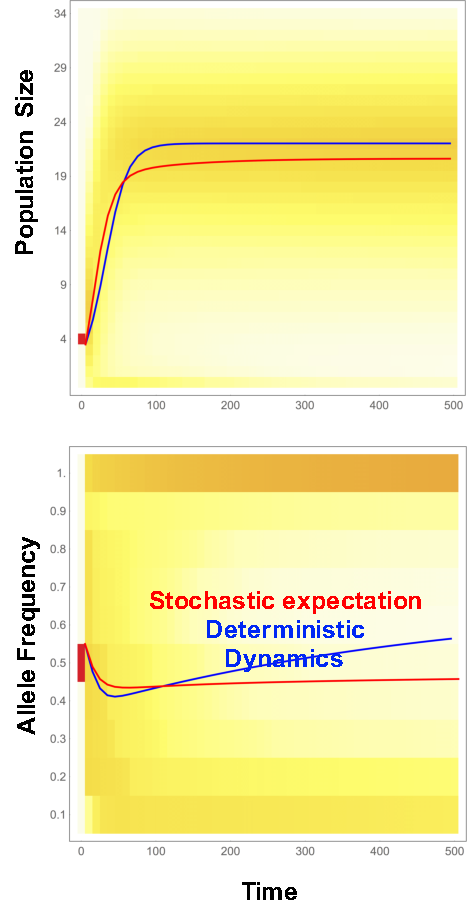
\includegraphics[width=0.7\columnwidth]{DensityDependence.pdf}
\end{center}
\end{minipage}%
\end{frame}
\end{document}